\documentclass[runningheads]{llncs}

%
\usepackage{graphicx}
\usepackage[utf8]{inputenc}
\usepackage[slovak]{babel}
\usepackage{multirow}
\PassOptionsToPackage{hyphens}{url}\usepackage{hyperref}
%
\begin{document}

\authorrunning{Jozef Varga}
\titlerunning{Využitie genetického algoritmu na výber funkcií v oblasti behaviorálnej biometrie}
%
\title{Využitie genetického algoritmu na výber funkcií v oblasti behaviorálnej biometrie}
%
%
\author{Jozef Varga}
%
\institute{Fakulta informatiky a informačných technológií STU v Bratislave, 
Ilkovičova 2, 842 16 Bratislava 4}
%
\maketitle              % typeset the header of the contribution
%
\begin{abstract}
    Výber funkcií je v strojovom učení náročnou kombinatorickou úlohou. 
    Funkcie, ktoré neskôr vstupujú do rôznych modelov v strojovom učení, majú
    veľký vplyv na následnú presnosť a rýchlosť samotného modelu. Toto je jeden z problémov,
    ktorý sa vyskytuje pri autorizovaní užívateľa pomocou behavioralnej biomerie. Práve pri
    zaznamenávaní dát o užívateľovy, získame veľké množstvo atributov, ktoré znižujú rýchlosť výpočtu
    a taktiež degradujú kvalitu klasifikácie. 
    
    V tomto článku sme vytvorily genetický algoritmus, ktorý používame práve na výber funkcií. Nami vytvorenú
    metódu porovnávame s bežnými metódami ako sú Variance Inflation Factor (VIF) a vyber funkcií pomocou korelácií. 
    Zvolené metódy boli porovnané pomocou rôznych klasifikátorov ako sú napríklad KNN, SVM, Naive Bayes a iné. 
    V práci sme využili verejný dataset~\cite{ref_dataset_anguita,ref_dataset} ktorý obsahuje biometrické dáta o 
    užívateľoch. Tieto dáta obsahujú informácie o tom v akom stave sa nachádza užívateľ, teda či leží, sedí, 
    kráča,  kráča hore schodmy, kráča dole schodmy alebo stojí.
    V tejto práci sa ukázalo, že použitie genetického algoritmu zlepšilo výsledky jednotlivých klasifikátorov.

\keywords{Behavioralna biometria \and Genetický algoritmus \and Strojové učenie \and Výber funkcií / atributov.}
\end{abstract}
%

%Úvod / Introduction - aká úloha sa ide riešiť, prečo je dobré ju riešiť
\section{Úvod}

V dnešnej dobe je využitie smartfónov na vzostupe. 
Veľké množstvo ľudí tieto zariadenia využíva aj na vyhľadávanie informácií, 
úpravu dokumentov a rôzne ďalšie funkcionality, 
ktoré tieto zariadenia podporujú~\cite{ref_bomhold}. 
To, že sú smartfóny veľkou súčasťou technologického sveta potvrdzuje aj 
štatistika z roku 2018, ktorá hovorí, že až 52,2\% 
zobrazení globálnych webových stránok prebiehalo pomocou mobilných zariadení. 
Zaujímavé je, že v tomto prípade ide o nárast až 51,5\% 
oproti štatistike z roku 2009~\cite{ref_statista19}. Mobilné zariadenie
prináša veľmi veľa nových možností výskumu ktoré sú orientované na správanie človeka.
Dôvodom je hlavne veľké množstvo informácií ktoré sú možné vďaka senzorom v mobilnom 
zariadenií zaznamenať. 

Tieto senzory zaznamenávajú takzvané biometricke črty.  
Biometria sa zakladá na charakteristických črtách konkrétnej osoby. Tieto biometrické 
črty sa delia na dva typy, a to na fyziologické a behaviorálne 
(viď. Obr.~\ref{fig_rozdelenie_biometrie}).~\cite{ref_teh} Fyziologická biometria, 
ako napríklad odtlačok prsta, je veľmi často využívanou overovacou technikou, 
keďže je jedinečná a stála. Táto biometria má však aj svoje nevýhody. 
DNA, čo je typickým príkladom tejto biometrie, je dosť invazívne na to, 
aby sa využívalo napríklad na smartfónoch, keďže jej využitie by 
vyžadovalo určitú podmienenú činnosť užívateľa, napríklad odber krvi. 
Naopak behaviorálna biometria má výhodu v možnosti práce na pozadí bez akejkoľvek 
určitej požadovanej činnosti užívateľa. Keďže sa jedná o charakteristiky, 
ako napríklad rýchlosť písania, nakláňanie smartfónu alebo chôdza, 
používateľove správanie môže byť overené počas bežných činností. ~\cite{ref_teh}
Výhodou behaviorálnych črt je teda fakt, 
že ak už zariadenie disponuje potrebným hardvérom, 
v prípade mobilných zariadeniach napríklad senzormi, 
je možné vykonávať rôzne opreácie ako napríklad autentifikáciu užívateľa alebo 
identifikovanie stavu v akom sa užívateľ nachádza bez toho, aby o 
tom samotný užívateľ vedel. Naopak nevýhodou tejto biometrie je, 
že behaviorálne charakteristiky užívateľa sa časom menia, 
a teda je potrebné častejšie vytvorenie profilu užívateľa ~\cite{ref_seyd}. 

Jedným z problémov ktorý sa objavuje pri prácach s behaviorálnimy črtamy, 
je množstvo atributov, ktoré sa získavajú zo senzorov.~\cite{ref_nascimento} 
Získané atributy môžu obsahovať irelevantné/zavádzajúce informácie, ktoré
môžu mať za následok zníženie kvality klasifikácie modelu.
~\cite{ref_babatunde,ref_lu,ref_nascimento,ref_smith,ref_zhao} 

Práve výberom atributov sa 
budeme v tejto práci bližšie zaoberať. Naša metóda na výber atributov spočíva vo využití 
genetického algoritmu, ktorý bude aplikovaný na výber čŕt v datasete ktorý sa venuje skúmaniu
stavu užívateľa (leží, chodí, sedí) na základe biometrických črt získaných z 
mobilného zariadenia.~\cite{ref_dataset_anguita,ref_dataset}


\begin{figure}
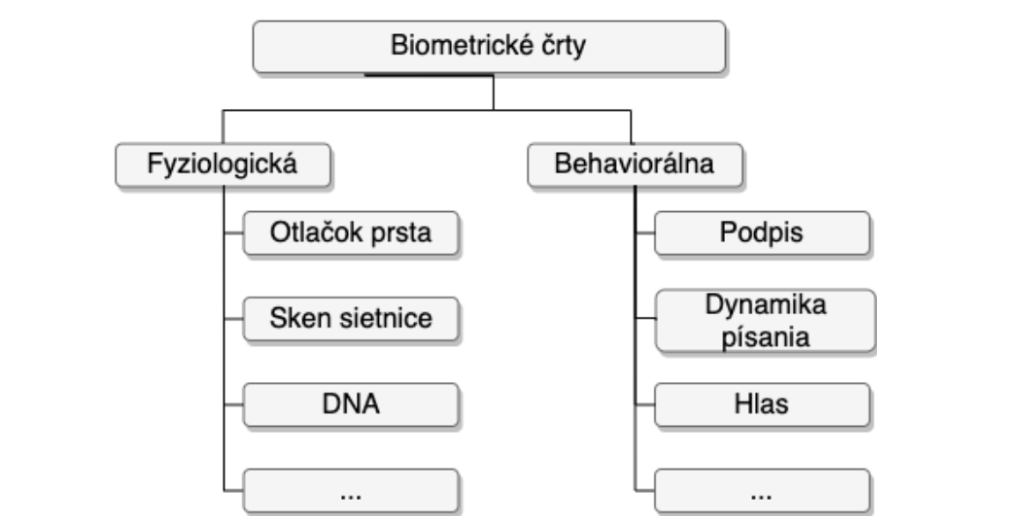
\includegraphics[width=\textwidth]{image/rozdelenie_biometrie.png}
\caption{Typy biometrických čŕt~\cite{ref_teh}} \label{fig_rozdelenie_biometrie}
\end{figure}

%Podobné práce / Related Work - ako riešili vašu alebo podobnú úlohu vexistujúcich prácach - nezabudnite v texte uvádzať citácie na práce.
\section{Podobné práce}

Výber atributou je veľmi podstatnou časťou pri strojovom učení. Veľmi veľa prác sa 
zaoberá rôznymi metódami ktoré by boli nápomocné pri spracovávaní rôznich datasetov.
V práci ~\cite{ref_nascimento} experimentovali nad dvoma databázami, pričom 
prvá databáza mala 43 atributov a 231 záznamov. Druhá databáza obsahovala žé atributov 
a 7555 záznamov. Dáta si rozdelily na testovaciu a trénovaciu množinu v pomere 66:33. 
Teda 66\% bolo dát bolo určených na trénovanie modelu a 33\% dát na jeho trénovanie. 
V práci využívajú na klasifikáciu modely KNN, SVM a Naive Bease (viď. Tab.~\ref{tab_vyber_funkci}). Na konci experimentu zhodnotili 
že využitie genetického algoritmu na vyber atributov pri rôznych klasifikátoroch mal veľmi priaznivé
účinky práve na SVM a to v zlepšení až o 14,55\% v prvom datasete a 11,77\% v druhom datasete.
Keďže zlepšenie bolo viditeľne vidieť pri každom zo spomenutých klasifikátorov, v práci usúdili že
využitie genetických algoritmov v tejto problematike zvyšuje presnosť klasifikátora. Naše riešenie chceme
porovnať s existujúcimi algoritmamy na výber funkcií a to variance inflation factor (VIF) a výber na 
základe korelácií.

\begin{table}[]
\centering
\caption{Accuracy (pesnosť ACC) modelov v percentách výberu funkcií.~\cite{ref_nascimento}}\label{tab_vyber_funkci}
\begin{tabular}{|c|c|c|c|}
\hline
                     & \multicolumn{3}{c|}{\textbf{Bez výberu funkcií}}                     \\ \hline
\textbf{Databáza}    & \textbf{KNN}          & \textbf{SVM}          & \textbf{Naive Bayes} \\ \hline
Da Silva et al. 2016 & 72.73 ±2.74           & 73.55 ±2.63           & 55.54±3.54           \\ \hline
Giot et al. 2009     & 86.72 ±0.58           & 78.28 ±0.67           & 69.33 ±0.67          \\ \hline
\textbf{Databáza}    & \multicolumn{3}{c|}{\textbf{Využitie genetického algoritmu na výber funkcií}} \\ \hline
Da Silva et al. 2016 & 87.85±0.84            & 88.10 ±0.90           & 81.64 ±0.97          \\ \hline
Giot et al. 2009     & 88.86 ±0.23           & 90.05±0.41            & 77.44 ±0.27          \\ \hline
\end{tabular}
\end{table}


V ďalšej práci\cite{ref_babatunde} využili na výber atributov tri rôzne algoritmy a to 
genetický algoritmus, WEKA-CFS a WEKA-ranker. Na vyhodnotenie taktiež použili viacero klasifikátorov
a to Multi-Layer Perceptron (MLP), Random Forest (RF), J48, Naive Bayes a regresiu. Najlepšie výsledky 
boli získané pomocou MLP. Ako najlepšia funkcia na výber atributov sa ukázal práve genetický algoritmus,
ktorý má výhodu práve v širokej možnosti nastavovania.

Nasledujúca práca\cite{ref_zhao} využila genetický algoritmus na optimalizáciu nie 
len výberu funkcií, ale aj výberu parametrov pre SVM klasifikátor. Výsledky im ukázali
, že využitie tohoto algoritmu, nie len zlepšilo výsledky klasifikácie, 
ale oproti využitia grid searchu aj zrýchlilo výpočet o 2,62 sekundy bez využitia
vyberu funkcií a o 1,21 sekundy rýchlejšia ak sa výber funkcií využil.
Presnosť klasifikácie sa zvýšila až o 3,57\%. 83,14 ± 7,19 boli najnižšie 
získané hodnoty s využitím výberu funkcií založených na genetickom algoritme.

Posledná skúmaná práca \cite{ref_smith} sa zaoberala predovsetkým klasifikátorom C4.5.
Skúmali ako vplýva genetický algoritmus, ktorého fitnes funkcia pozostáva na strome, 
na výber funkcií aj u iných algoritmov. Teda neskúšali využívať vo fitnes funkcii len
klasifikátor s ktorým neskôr prebieha klasifikácia. Zistili že takáto fitnes funkcia,
taktiež zlepšuje aj iné modely. Ich výsledky sa ukázali ak rovnakú funkciu použili na 
Naive Bayes kde sa klasifikácia zlepšila o 4,92 \%.


%opis použitého algoritmu - aj s odôvodnením výberu algoritmu
\section{Využívané algoritmy na výber funkcií}
V tejto práci sme sa rozhodli porovnať genetický algoritmus na výber funkcií s
algoritmamy Variance Inflation Factor a Výber funkcií pomocou korelácií. Tieto 
algoritmy sa radia medzi základné algoritmy na výber funkcií. \cite{ref_xu}
\subsection{Variance Inflation Factor}
Tento algoritmus odstranuje funkcie ktoré majú veľmmi silnú kolinearitu.
Vif odhaduje do akej miery je rozptyl koeficientu zväčšený kôli linearnej závislosti
s inou prediktorom. Výpočet VIF pre každý stĺpec sa dá získať vykonaním lineárnej 
regresie tohoto stĺpca s všetkými ostatnými stĺpcami.\cite{ref_xu}
Vzorec pre výpočet VIF vyzerá nasledujúco:
\begin{equation}
VIF_{i}=\frac{1}{1-R_{i}^{2}}
\end{equation}    
V uvedenom vzorci \begin{math}R_i^2\end{math} predstavuje koeficint regresie medzi i-tou premennou a 
všetkými ostatnými premennými. VIF sa pri výbere funkcí porovnáva a odstranujú sa hraničné hodnoty.\cite{ref_xu}

\subsection{Výber funkcií pomocou korelácií}
Funkcie sú vyberaná pomocou korelačného koeficientu. Koeficient korelácie je miera linearnej intenzity 
korelácie. Najčastejšie je využívaný Pearsonov korelačný koeficient. Tento koeficient nadobúda hodnoty medzi
\begin{math}1\end{math} až \begin{math}-1\end{math}. \begin{math}1\end{math} vo výsledku predstavuje perfektú pozitívnu 
koreláciu (podobnosť). Naopak \begin{math}-1\end{math} predstavuje 
perfektńu negatívnu koreláciu (podobnosť). \begin{math}0\end{math} označuje, že medzi prvkami nie je žiadna korelácia / podobnosť.
Ak prebieha výbere funkcií touto metódou, vďaka výsledkom korelácie sa odstráňuju veľmi podobné funkcie.\cite{ref_xu}

\subsection{Genetický algoritmus}

Genetické algoritmy sú inšpirované evolúciou. Teda ich základ sa skladá z generácií ktoré sa vyvíjajú a obsahujú 
určité množstvo chromozómv, ktoré sa spolu volajú populácia. Tieto chromozómy obsahujú kritické informácie 
potrebné na vyriešenie problému. Tieto algoritmy sa využívaju najme na optimalizáciu rôznich
problémov. Ich uplatnenie je v praxi veľmi široké.\cite{ref_babatunde,ref_whitley} Nami vytvorený algoritmu začína 
inicializáciou populácie genetického algoritmu (viď. Obr.~\ref{fig_ga_rozdelenie}).

\begin{figure}
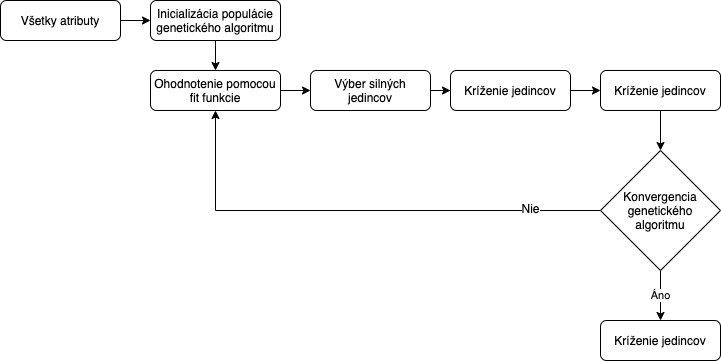
\includegraphics[width=\textwidth]{image/GA_alg.png}
\caption{Schéma genetického algoritmu na výber funkcií} \label{fig_ga_rozdelenie}
\end{figure}
    
\subsubsection{Inicializácia populácie genetického algoritmu.}

Pri inicializácií sa nastavia prvotné nastavenia genetického algoritmu (viď. Tab.~\ref{tab_nastavenie_gen_alg}). 
V algoritme je chromozóm reprezentovaný \begin{math}n\end{math} génmy. Jeden gén prezentuje \begin{math}1\end{math} 
alebo \begin{math}0\end{math} ktorá hovorý či vo výslednom vektore funkcií sa táto funkcia nachádza alebo nie. 
Počet tých to génov \begin{math}n\end{math} je počtom funkcií ktoré sú vo vstupnom vektore. Teda 
koľko funkcií má daný dataset.

\begin{table}[]
\centering
\caption{Nastavenie genetického algoritmu}\label{tab_nastavenie_gen_alg}
\begin{tabular}{|l|l|}
\hline
\textbf{Parametre GA}                    & \textbf{hodnota}  \\ \hline
Fit funkcia založená na modely           & AdaBoost \\ \hline
Reprezentácia génu                       & Boolean  \\ \hline
Maximálny počet generácií                & 20       \\ \hline
Veľkosť populácie                        & 100      \\ \hline
Chromozómy vytvorené krížením            & 30       \\ \hline
Chromozómy vytvorené generovaním         & 30       \\ \hline
Najlepšie chromozómy z minulej generácie & 30       \\ \hline
Percentuálna šanca mutácie a kríženia    & 60\%     \\ \hline
\end{tabular}
\end{table}

\subsubsection{Ohodnotenie populácie pomocou fit funkcie.}

Populácia ktorá sa dostane do tohoto kroku, musí byť ohodnoťená pomocou fit (fitnes) funkcie. 
Táto funkcia musí odlišovať jednotlivé chromozómy tak, aby bolo možné ich porovnať a zistiť, ktorý
z týchto chromozómov je najúspešnejší. Táto fit funkcia pozostáva z priemeru päť násobnej crossvalidacie ktorej jadro
je vytvorené z AdaBoost. Najlepšie hodnotený chromozóm sa uloží a algoritmus pokračuje
na výber jedincov (chromozómov) do ďalšej generácie.

\subsubsection{Výber silných jedincov.}

Tento spôsob sa nazýva elitárstvo. Teda koľko najlepších chromozómov z predchádzajúcej generácie prejde
do novej generácie. Výhodou je najme to, že silné jedince sa nadalej reprodukujú a predávajú svoje vlastnosti
novo vytvoreným chromozómom.

\subsubsection{Kríženie jedincov.}

Pri krýžení sa spájajú vlastnosti dvoch jedincov do jedného (viď. Obr.~\ref{fig_ga_krizenie}).
Do kríženia vstupujú dva chromozómy ktoré majú zrkadlové postavenie v liste ktorý je zoradený podľa fit funkcie. 
Jeden z časti kde je fit funkcia najsilnejšia a jeden z časti kde je fit funkcia naopak slabšia. 
Tento spôsob by mal pomôcť algoritmu zastať na lokálnom maxime. Následne sa prechádza po génoch 
jednotlivých chromozómov a podľa percentuálnej náhody sa vyberie jeden z génov do budúceho jedinca.
Šanca s akou sa jednotlivé gény volia ako aj počet takto vytvorených jedincov sa v genetickom algoritme
nastavuje pomocou parametrov (viď. Tab.~\ref{tab_nastavenie_gen_alg}). 

\begin{figure}
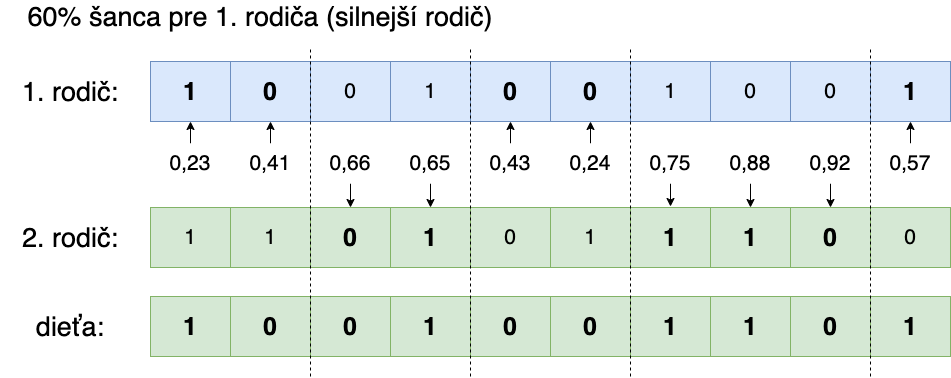
\includegraphics[width=\textwidth]{image/krizenie.png}
\caption{Kríženie chromozómov} \label{fig_ga_krizenie}
\end{figure}

Zvyšné chromozómy sa náhodne vygenerujú ako pri inicializácií aby počet chromozómov v každej generácií bol rovnaky. 
Ako posledné prejde algoritmus k mutácií. Tá prejde všetky chromozómy v zadanej populácií a prechádza jednotlivé gény.
Nad každým génom vygenerujé náhodné číslo ktoré s 60\% šancov zmení gén na opačný (viď. Obr.~\ref{fig_ga_mutovanie}). 

\begin{figure}
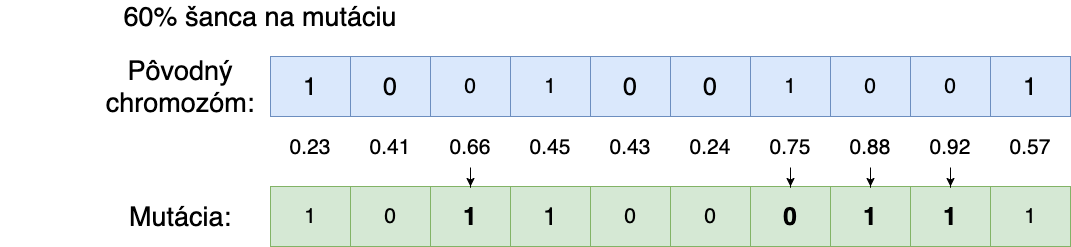
\includegraphics[width=\textwidth]{image/mutacia.png}
\caption{Mutovanie chromozómov} \label{fig_ga_mutovanie}
\end{figure}


%opis vykonaných experimentov - opis použitého datasetu, opis cieľu a postupuexperimentu, opis nastavení algoritmu (odôvodnenie prečo zvolené nastavenia), opis metrík, ktorými experiment vyhodnocujete... ak sa porovnávate s existujúcimi riešeniami, nezabudnite ich citovať, prípadne aj stručne opísať
\section{Experimenty}

Zvolená konfigurácia genetického algoritmu zobrazená v tabuľke ~\ref{tab_nastavenie_gen_alg} bola zvolená na 
základe pilotných testov nad rôznimy datami. V experimente využijeme dataset ktorý obsahuje behaviorálne 
záznamy z mobilného zariadenia~\cite{ref_dataset_anguita,ref_dataset}. Tento dataset je slúži na klasifikovanie
stavu používateľa. Teda či používateľ leží, sedí, kráča, kráča hore schodmy, kráča dole schodmy alebo stojí.
Dataset obsahuje informácie o 30 dobrovolníkoch vo veku 19 až 48 rokov. Každý používateľ vykonal spomenutých
6 aktivít pri ktorých mal na páse pripevnený smartfón Samsung Galaxy S II. Dataset obsahuje informácie z 
gyroskopu a akcelerometra. Z nich sa zaznamenávalo 3-osové lineárne zrýchlenie a 3-osové uhlové rýchlosti 
pri konštantnej rýchlosti 50 Hz. V datasete sa nachádza 3609 záznamov. Pre každý záznam v datasete sa poskytuje 
vektorom s 561 funkciami, ktoré obsahujú:

\begin{itemize}
\item trojosové zrýchlenie z akcelerometra a odhadované zrýchlenie tela
\item Trojosová uhlová rýchlosť z gyroskopu
\item Označenie činnosti
\item Označenie konkrétneho subjektu
\end{itemize}

Nad týmto datasetom sa snažíme overiť a porovnať silu genetický algoritmu s tým, že porovnávame 
jeho získané skóre so skóre, ktoré získa algoritmus VIF alebo analýza na základe korelácií. Skóre sa 
vypočítavalo ako fit funkcia. Teda 5 násobnou validaciou. Modely ktoré sme využili v experimente boli 
AdaBoost, Decision Tree, Extra Trees, Naive Bayes, Nearest Neighbors, Linear Discriminant Analysis, 
Logistic Regression, Neural Net, Random Forest, SVM Sigmoid, SVM RBF, QDA.

%Vyhodnotenie / Evaluation - prehľadné výsledky experimentov (formou textového opisu, grafov, tabuliek, ...)
\section{Vyhodnotenie}

%Záver / Conclusion
\section{Záver}

%Použitá literatúra / References - používajte LNCS štýl odkazovania sa nazdroje, pokyny nájdete aj v šablóne
\begin{thebibliography}{8}

\bibitem{ref_dataset_anguita}
Anguita, D. et al.: A public domain dataset for human activity recognition using smartphones. ESANN 2013 proceedings, 21st Eur. Symp. Artif. Neural Networks, Comput. Intell. Mach. Learn. April, 437–442 (2013).

\bibitem{ref_babatunde}
Babatunde, O. et al.: A Genetic Algorithm-Based Feature Selection. Int. J. Electron. Commun. Comput. Eng. 5, 4, 899–905 (2014).

\bibitem{ref_bomhold}
Bomhold, C.R.: Educational use of smart phone technology: A survey of mobile phone application use by undergraduate university students. Program. 47, 4, 424–436 (2013). \doi{10.1108/PROG-01-2013-0003}.

\bibitem{ref_lu}
Lu, H. et al.: A hybrid feature selection algorithm for gene expression data classification. Neurocomputing. 256, 2017, 56–62 (2017). \doi{10.1016/j.neucom.2016.07.080}.

\bibitem{ref_nascimento}
Nascimento, L.D.O. et al.: An investigation of genetic algorithm-based feature selection techniques applied to keystroke dynamics biometrics An investigation of genetic algorithm-based feature selection techniques applied to keystroke dynamics biometrics. SBSeg, 2–5 (2019).

\bibitem{ref_smith}
Smith, M.G., Bull, L.: Genetic programming with a genetic algorithm for feature construction and selection. Genet. Program. Evolvable Mach. 6, 3, 265–281 (2005). \doi{10.1007/s10710-005-2988-7}.

\bibitem{ref_seyd}
Syed, Z. et al.: Touch gesture-based authentication on mobile devices: The effects of user posture, device size, configuration, and inter-session variability. J. Syst. Softw. 149, 158–173 (2019). \doi{10.1016/j.jss.2018.11.017}.

\bibitem{ref_statista19}
statista.com, 2018. Percentage of all global web pages served to mobile phones from 2009 to 2018. \url{https://www.statista.com/statistics/241462/global-mobile-phone-website-traffic-share/}. Posledny prístup 10 Marca 2020

\bibitem{ref_teh}
Teh, P.S. et al.: A survey of keystroke dynamics biometrics. Sci. World J. 2013, (2013). \doi{10.1155/2013/408280}.

\bibitem{ref_dataset}
UC Irvine Machine Learning Repository, \url{https://archive.ics.uci.edu/ml/datasets/human+activity+recognition+using+smartphones}. Posledny prístup 10 Marca 2020

\bibitem{ref_whitley}
Whitley, D.: A genetic algorithm tutorial. Stat. Comput. 4, 2, 65–85 (1994). \doi{10.1007/BF00175354}.

\bibitem{ref_xu}
Xu, J. et al.: Methods for performing dimensionality reduction in hyperspectral image classification. (2018). \doi{10.1177/0967033518756175}.

\bibitem{ref_zhao}
Zhao, M. et al.: Feature selection and parameter optimization for support vector machines: A new approach based on genetic algorithm with feature chromosomes. Expert Syst. Appl. 38, 5, 5197–5204 (2011). \doi{10.1016/j.eswa.2010.10.041}.

\end{thebibliography}

\end{document}
